\chapter{Estadísticas de los operadores}
\label{apendice:estadisticas-operadores}
\begin{figure}[!ht]
\centering
    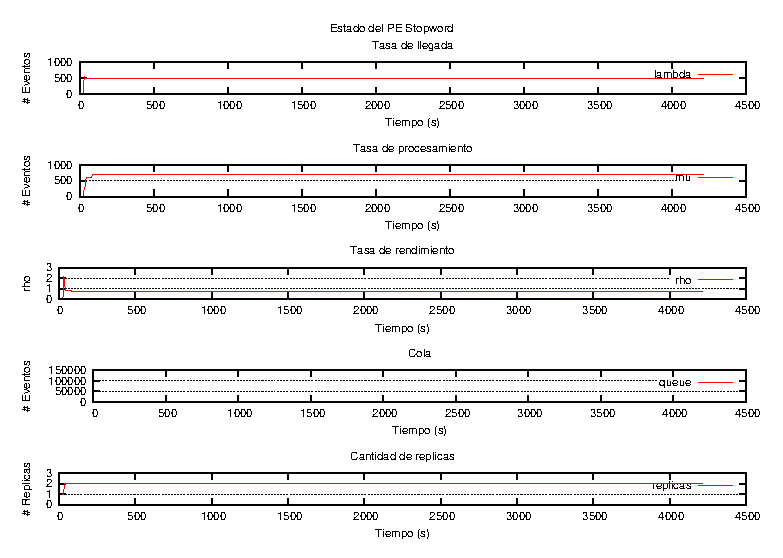
\includegraphics[scale=1]{images/exp/app1/uniform/cm/statusStopwordPE.eps}
    \caption{Estadísticas del PE Stopword en la primera aplicación con un envío constante de la fuente de datos con uso del modelo.}
    \label{fig:app1-uniform-statusStopwordPE-cm}
\end{figure}

\begin{figure}[!ht]
\centering
    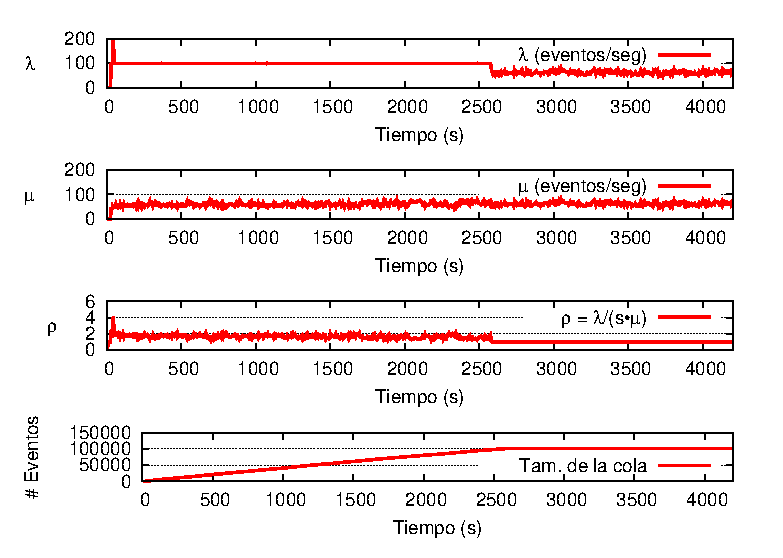
\includegraphics[scale=1]{images/exp/app1/uniform/sm/statusStopwordPE.eps}
    \caption{Estadísticas del PE Stopword en la primera aplicación con un envío constante de la fuente de datos sin uso del modelo.}
    \label{fig:app1-uniform-statusStopwordPE-sm}
\end{figure}

\begin{figure}[!ht]
\centering
    \includegraphics[scale=1.1]{images/exp/app1/uniform/cm/statusLanguagePE.eps}
    \caption{Estadísticas del PE Language en la primera aplicación con un envío constante de la fuente de datos con uso del modelo.}
    \label{fig:app1-uniform-statusLanguagePE-cm}
\end{figure}

\begin{figure}[!ht]
\centering
    \includegraphics[scale=1.1]{images/exp/app1/uniform/sm/statusLanguagePE.eps}
    \caption{Estadísticas del PE Language en la primera aplicación con un envío constante de la fuente de datos sin uso del modelo.}
    \label{fig:app1-uniform-statusLanguagePE-sm}
\end{figure}

\begin{figure}[!ht]
\centering
    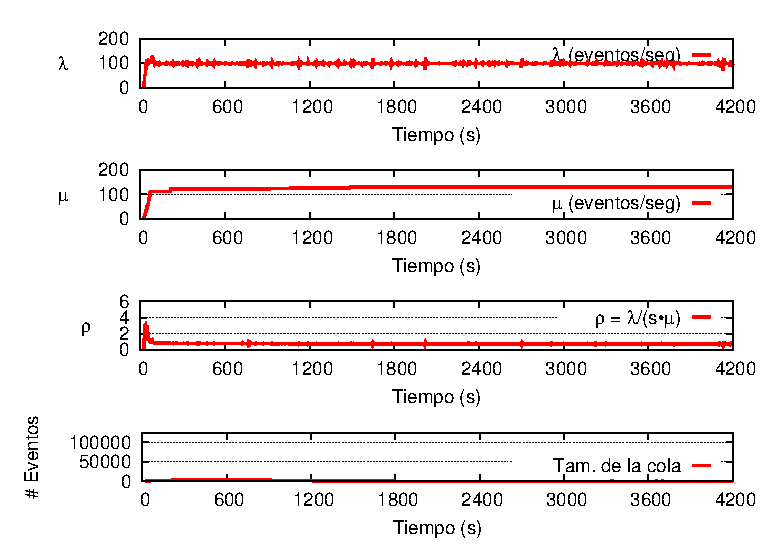
\includegraphics[scale=1.1]{images/exp/app1/uniform/cm/statusCounterPE.eps}
    \caption{Estadísticas del PE Counter en la primera aplicación con un envío constante de la fuente de datos con uso del modelo.}
    \label{fig:app1-uniform-statusCounterPE-cm}
\end{figure}

\begin{figure}[!ht]
\centering
    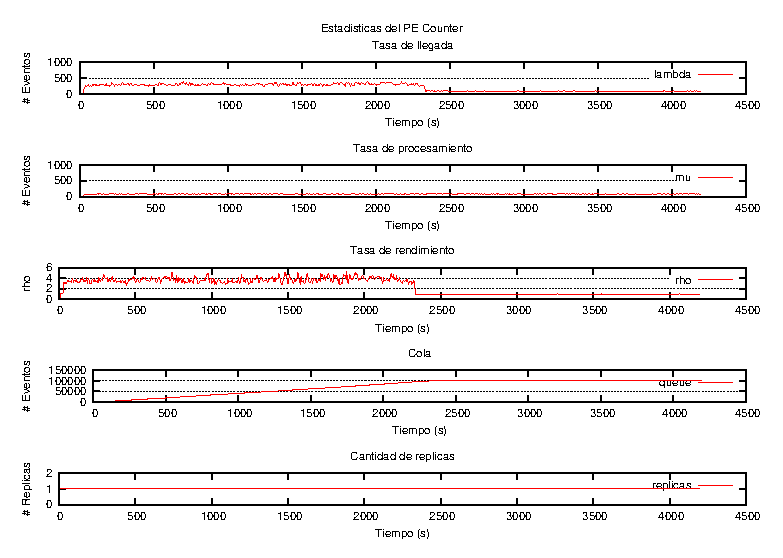
\includegraphics[scale=1.1]{images/exp/app1/uniform/sm/statusCounterPE.eps}
    \caption{Estadísticas del PE Counter en la primera aplicación con un envío constante de la fuente de datos sin uso del modelo.}
    \label{fig:app1-uniform-statusCounterPE-sm}
\end{figure}

\begin{figure}[!ht]
\centering
    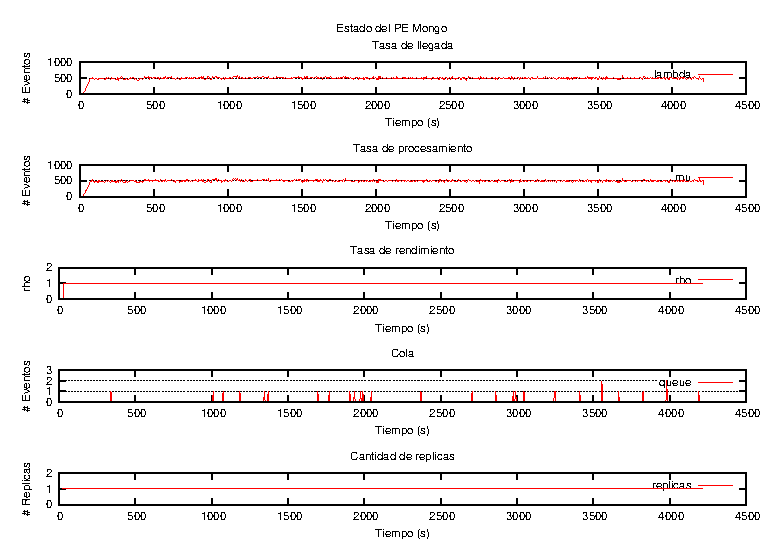
\includegraphics[scale=1.1]{images/exp/app1/uniform/cm/statusMongoPE.eps}
    \caption{Estadísticas del PE Mongo en la primera aplicación con un envío constante de la fuente de datos con uso del modelo.}
    \label{fig:app1-uniform-statusMongoPE-cm}
\end{figure}

\begin{figure}[!ht]
\centering
    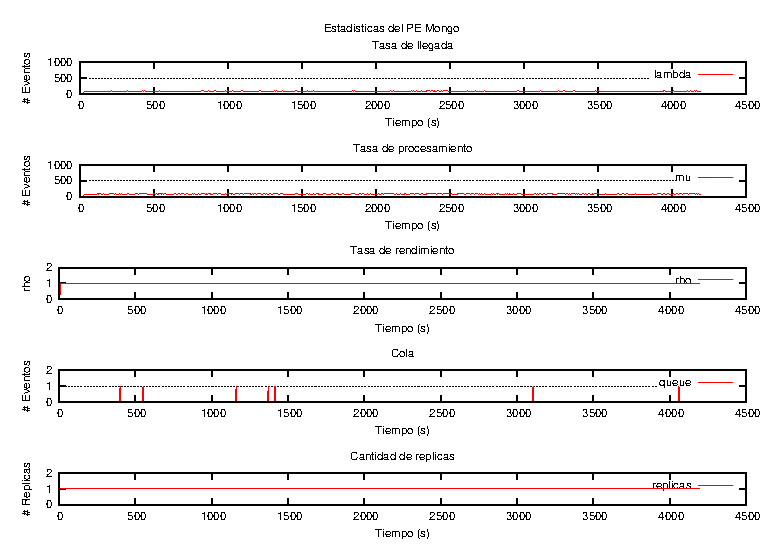
\includegraphics[scale=1.1]{images/exp/app1/uniform/sm/statusMongoPE.eps}
    \caption{Estadísticas del PE Mongo en la primera aplicación con un envío constante de la fuente de datos sin uso del modelo.}
    \label{fig:app1-uniform-statusMongoPE-sm}
\end{figure}

\begin{figure}[!ht]
\centering
    \includegraphics[scale=1.1]{images/exp/app1/normal/cm/statusStopwordPE.eps}
    \caption{Estadísticas del PE Stopword en la primera aplicación con un envío variable de la fuente de datos con uso del modelo.}
    \label{fig:app1-normal-statusStopwordPE-cm}
\end{figure}

\begin{figure}[!ht]
\centering
    \includegraphics[scale=1.1]{images/exp/app1/normal/sm/statusStopwordPE.eps}
    \caption{Estadísticas del PE Stopword en la primera aplicación con un envío variable de la fuente de datos sin uso del modelo.}
    \label{fig:app1-normal-statusStopwordPE-sm}
\end{figure}

\begin{figure}[!ht]
\centering
    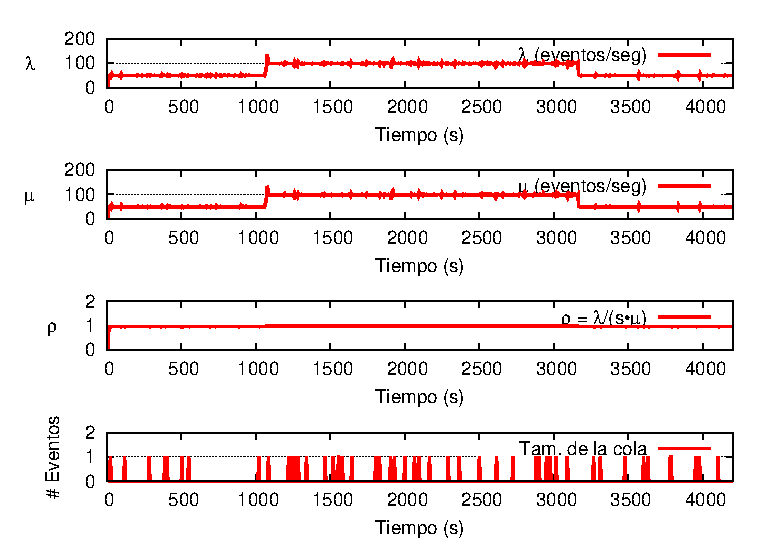
\includegraphics[scale=1.1]{images/exp/app1/normal/cm/statusLanguagePE.eps}
    \caption{Estadísticas del PE Language en la primera aplicación con un envío variable de la fuente de datos con uso del modelo.}
    \label{fig:app1-normal-statusLanguagePE-cm}
\end{figure}

\begin{figure}[!ht]
\centering
    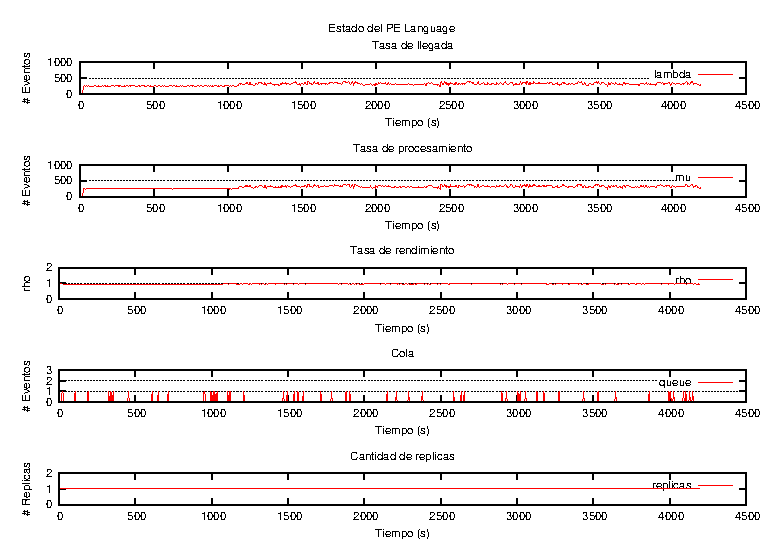
\includegraphics[scale=1.1]{images/exp/app1/normal/sm/statusLanguagePE.eps}
    \caption{Estadísticas del PE Language en la primera aplicación con un envío variable de la fuente de datos sin uso del modelo.}
    \label{fig:app1-normal-statusLanguagePE-sm}
\end{figure}

\begin{figure}[!ht]
\centering
    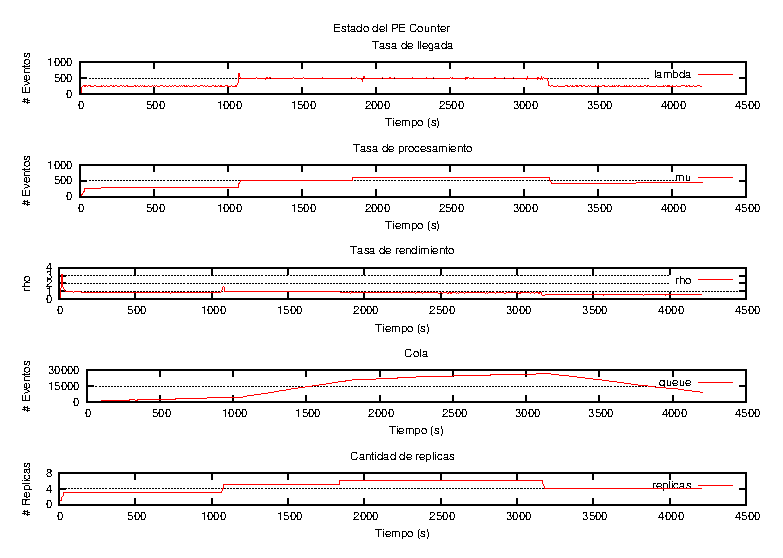
\includegraphics[scale=1.1]{images/exp/app1/normal/cm/statusCounterPE.eps}
    \caption{Estadísticas del PE Counter en la primera aplicación con un envío variable de la fuente de datos con uso del modelo.}
    \label{fig:app1-normal-statusCounterPE-cm}
\end{figure}

\begin{figure}[!ht]
\centering
    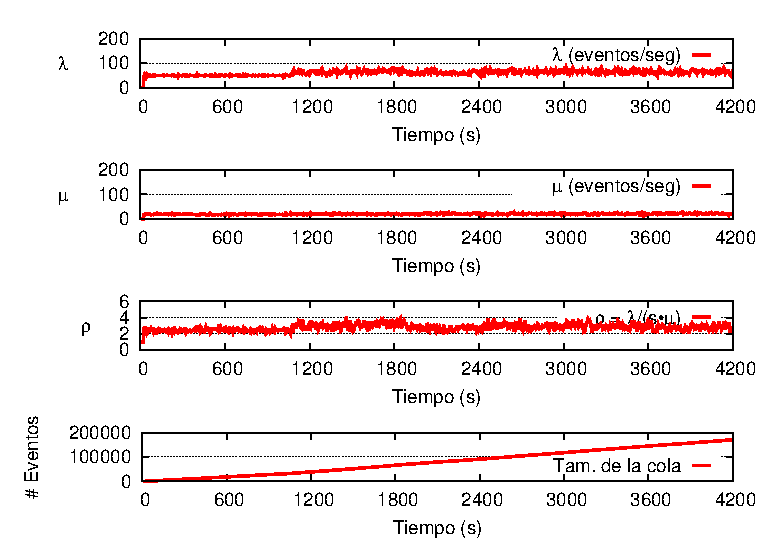
\includegraphics[scale=1.1]{images/exp/app1/normal/sm/statusCounterPE.eps}
    \caption{Estadísticas del PE Counter en la primera aplicación con un envío variable de la fuente de datos sin uso del modelo.}
    \label{fig:app1-normal-statusCounterPE-sm}
\end{figure}

\begin{figure}[!ht]
\centering
    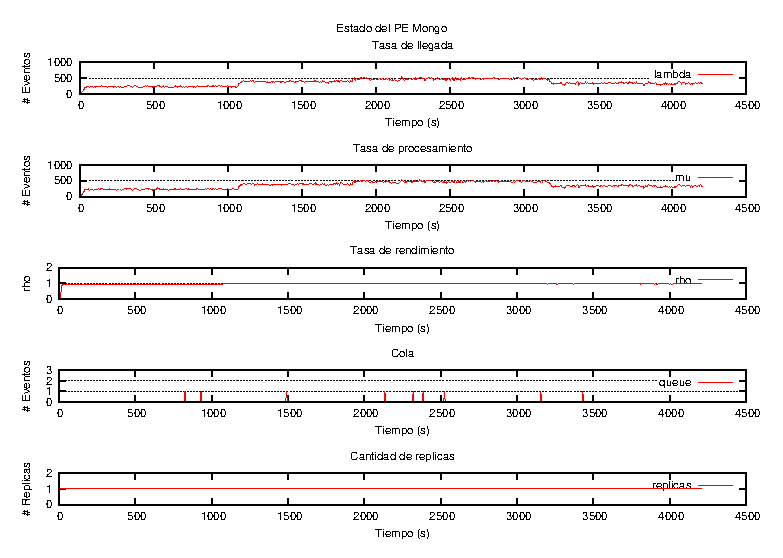
\includegraphics[scale=1.1]{images/exp/app1/normal/cm/statusMongoPE.eps}
    \caption{Estadísticas del PE Mongo en la primera aplicación con un envío variable de la fuente de datos con uso del modelo.}
    \label{fig:app1-normal-statusMongoPE-cm}
\end{figure}

\begin{figure}[!ht]
\centering
    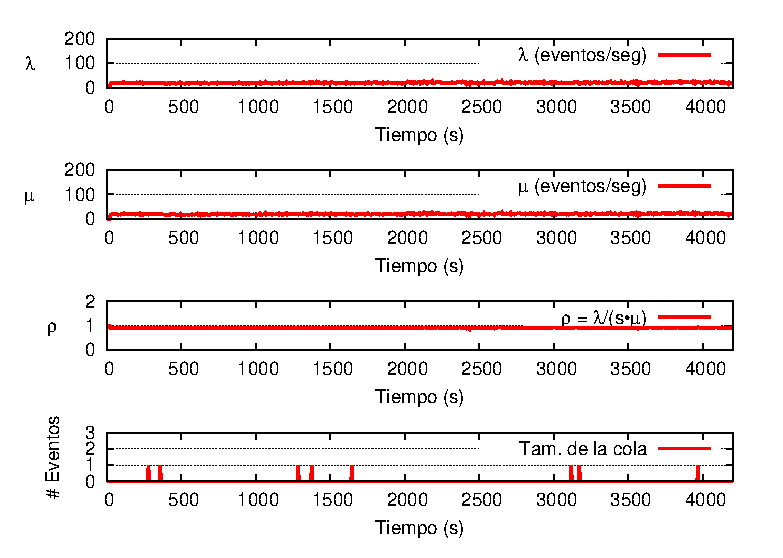
\includegraphics[scale=1.1]{images/exp/app1/normal/sm/statusMongoPE.eps}
    \caption{Estadísticas del PE Mongo en la primera aplicación con un envío variable de la fuente de datos sin uso del modelo.}
    \label{fig:app1-normal-statusMongoPE-sm}
\end{figure}

\begin{figure}[!ht]
\centering
    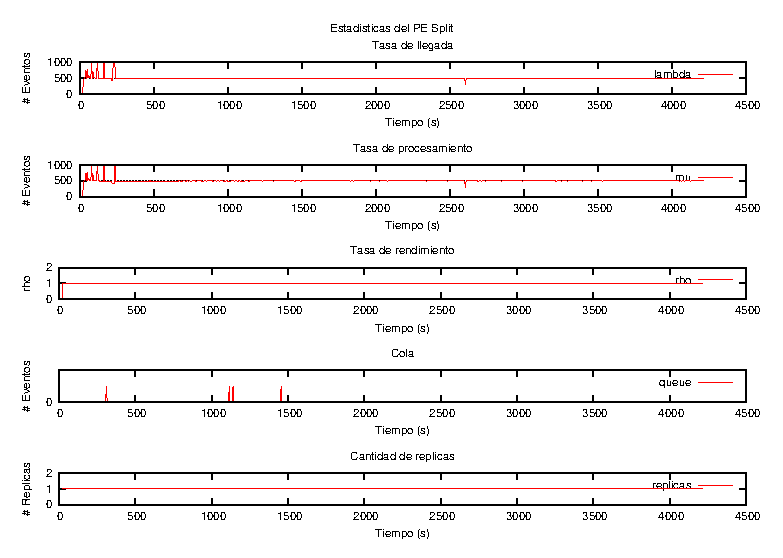
\includegraphics[scale=1.1]{images/exp/app2/uniform/cm/statusSplitPE.eps}
    \caption{Estadísticas del PE Split en la segunda aplicación con un envío constante de la fuente de datos con uso del modelo.}
    \label{fig:app2-uniform-statusSplitPE-cm}
\end{figure}

\begin{figure}[!ht]
\centering
    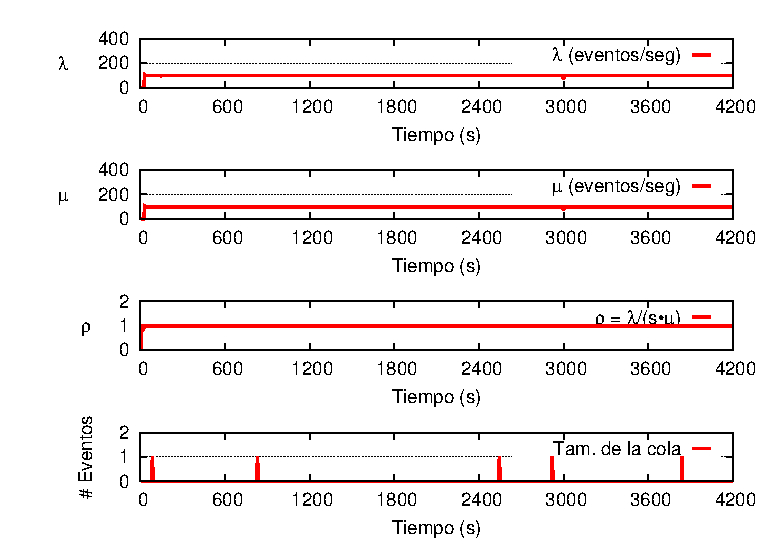
\includegraphics[scale=1.1]{images/exp/app2/uniform/sm/statusSplitPE.eps}
    \caption{Estadísticas del PE Split en la segunda aplicación con un envío constante de la fuente de datos sin uso del modelo.}
    \label{fig:app2-uniform-statusSplitPE-sm}
\end{figure}

\clearpage

\begin{figure}[!ht]
\centering
    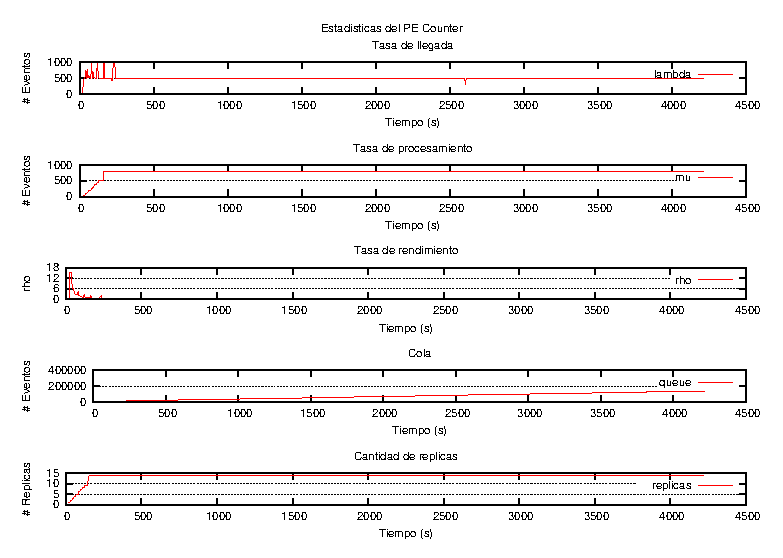
\includegraphics[scale=1]{images/exp/app2/uniform/cm/statusCounterPE.eps}
    \caption{Estadísticas del PE Counter en la segunda aplicación con un envío constante de la fuente de datos con uso del modelo.}
    \label{fig:app2-uniform-statusCounterPE-cm}
\end{figure}

\begin{figure}[!ht]
\centering
    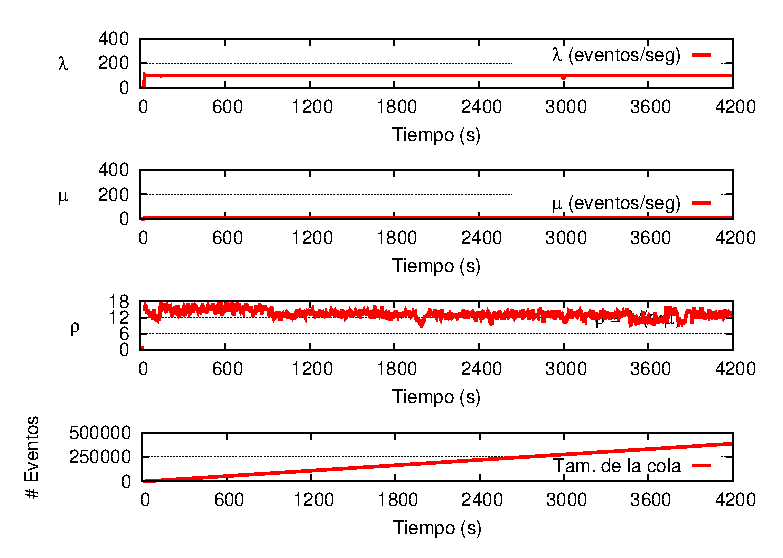
\includegraphics[scale=1]{images/exp/app2/uniform/sm/statusCounterPE.eps}
    \caption{Estadísticas del PE Counter en la segunda aplicación con un envío constante de la fuente de datos sin uso del modelo.}
    \label{fig:app2-uniform-statusCounterPE-sm}
\end{figure}

\begin{figure}[!ht]
\centering
    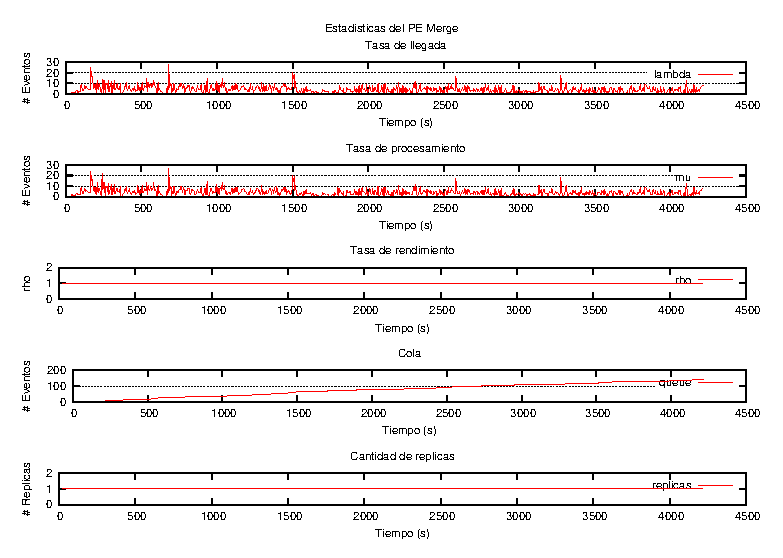
\includegraphics[scale=1.1]{images/exp/app2/uniform/cm/statusMergePE.eps}
    \caption{Estadísticas del PE Merge en la segunda aplicación con un envío constante de la fuente de datos con uso del modelo.}
    \label{fig:app2-uniform-statusMergePE-cm}
\end{figure}

\begin{figure}[!ht]
\centering
    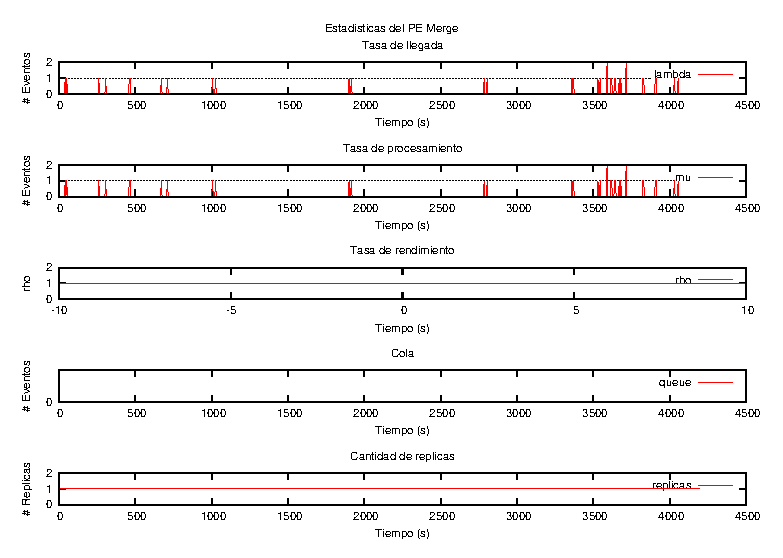
\includegraphics[scale=1.1]{images/exp/app2/uniform/sm/statusMergePE.eps}
    \caption{Estadísticas del PE Merge en la segunda aplicación con un envío constante de la fuente de datos sin uso del modelo.}
    \label{fig:app2-uniform-statusMergePE-sm}
\end{figure}

\begin{figure}[!ht]
\centering
    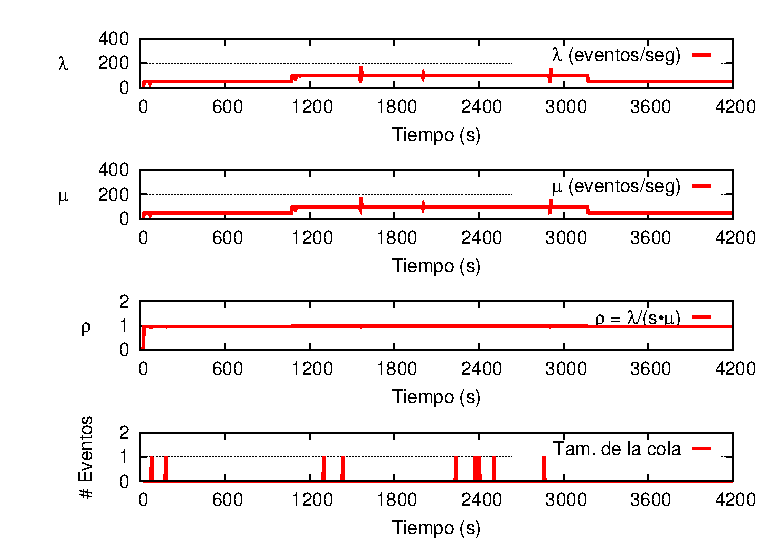
\includegraphics[scale=1.1]{images/exp/app2/normal/cm/statusSplitPE.eps}
    \caption{Estadísticas del PE Split en la segunda aplicación con un envío variable de la fuente de datos con uso del modelo.}
    \label{fig:app2-normal-statusSplitPE-cm}
\end{figure}

\begin{figure}[!ht]
\centering
    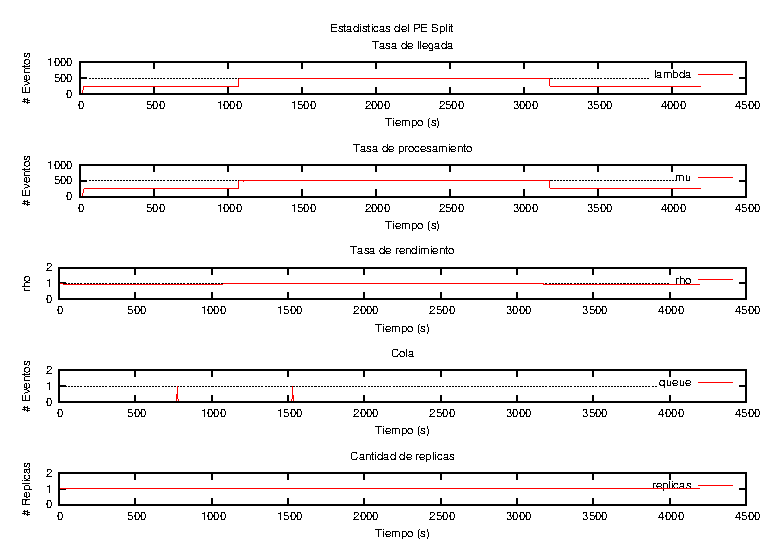
\includegraphics[scale=1.1]{images/exp/app2/normal/sm/statusSplitPE.eps}
    \caption{Estadísticas del PE Split en la segunda aplicación con un envío variable de la fuente de datos sin uso del modelo.}
    \label{fig:app2-normal-statusSplitPE-sm}
\end{figure}

\begin{figure}[!ht]
\centering
    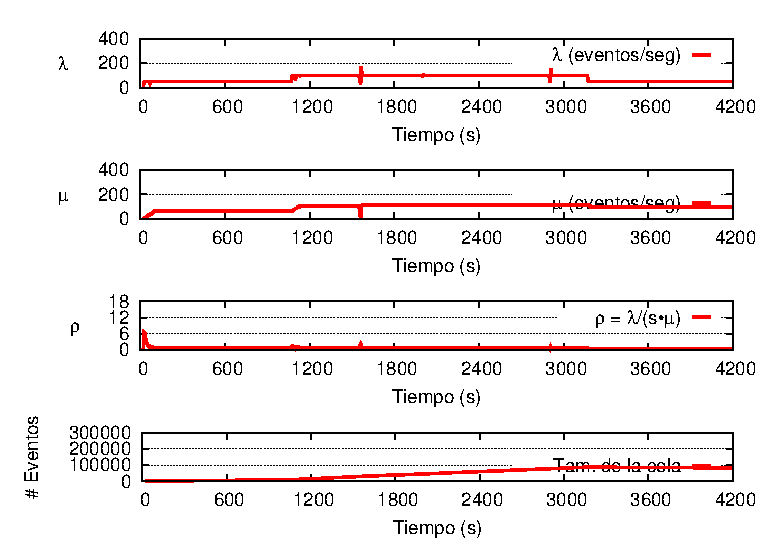
\includegraphics[scale=1.1]{images/exp/app2/normal/cm/statusCounterPE.eps}
    \caption{Estadísticas del PE Counter en la segunda aplicación con un envío variable de la fuente de datos con uso del modelo.}
    \label{fig:app2-normal-statusCounterPE-cm}
\end{figure}

\begin{figure}[!ht]
\centering
    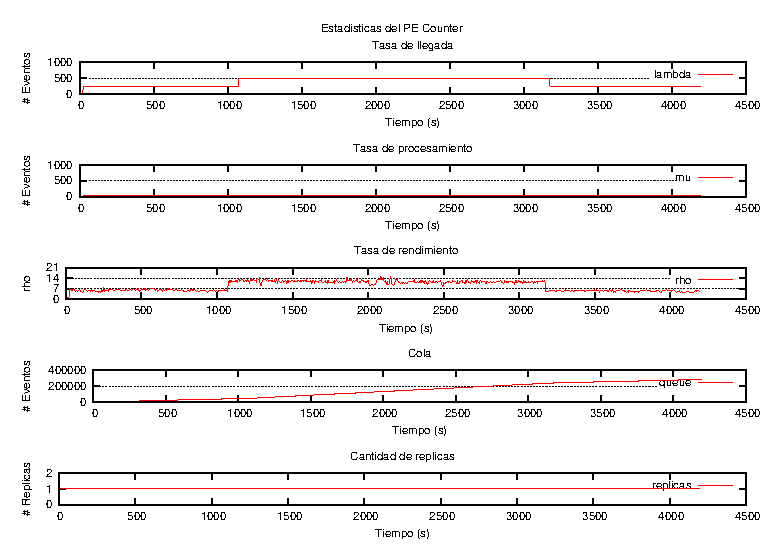
\includegraphics[scale=1.1]{images/exp/app2/normal/sm/statusCounterPE.eps}
    \caption{Estadísticas del PE Counter en la segunda aplicación con un envío variable de la fuente de datos sin uso del modelo.}
    \label{fig:app2-normal-statusCounterPE-sm}
\end{figure}

\begin{figure}[!ht]
\centering
    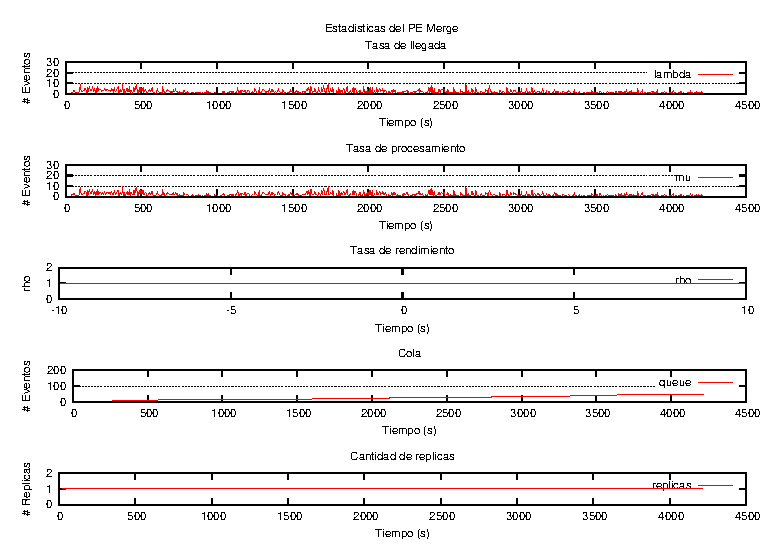
\includegraphics[scale=1.1]{images/exp/app2/normal/cm/statusMergePE.eps}
    \caption{Estadísticas del PE Merge en la segunda aplicación con un envío variable de la fuente de datos con uso del modelo.}
    \label{fig:app2-normal-statusMergePE-cm}
\end{figure}

\begin{figure}[!ht]
\centering
    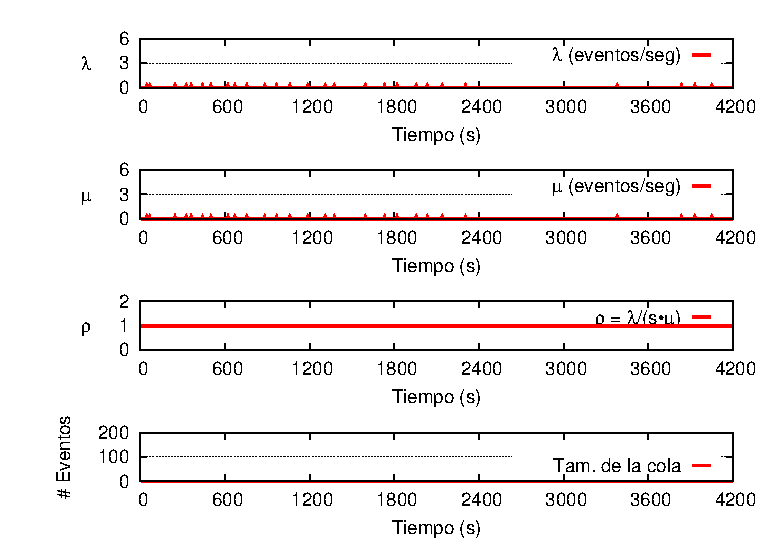
\includegraphics[scale=1.1]{images/exp/app2/normal/sm/statusMergePE.eps}
    \caption{Estadísticas del PE Merge en la segunda aplicación con un envío variable de la fuente de datos sin uso del modelo.}
    \label{fig:app2-normal-statusMergePE-sm}
\end{figure}

\begin{figure}[!htp]
\centering
    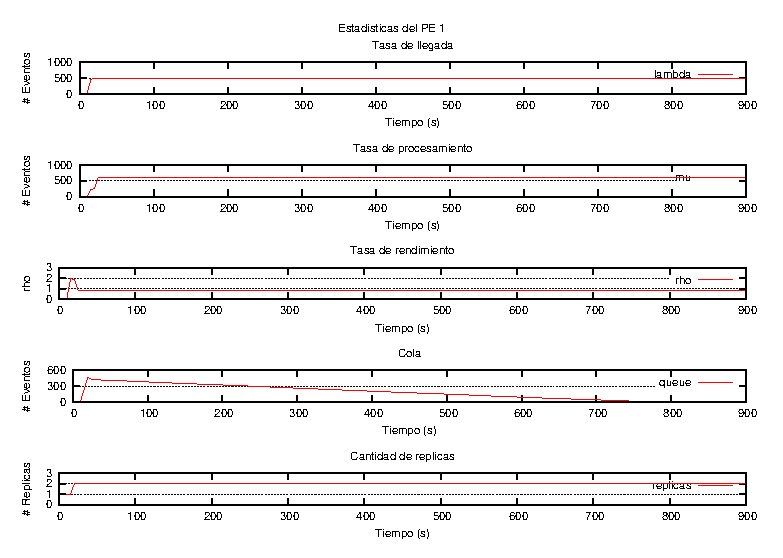
\includegraphics[scale=1]{images/exp/app3/cm/logical/statusOnePE.eps}
    \caption{Estadísticas del primer PE en la tercera aplicación con un envío constante de la fuente de datos con uso del modelo.}
    \label{fig:app3-statusOnePE-cm}
\end{figure}

\begin{figure}[!htp]
\centering
    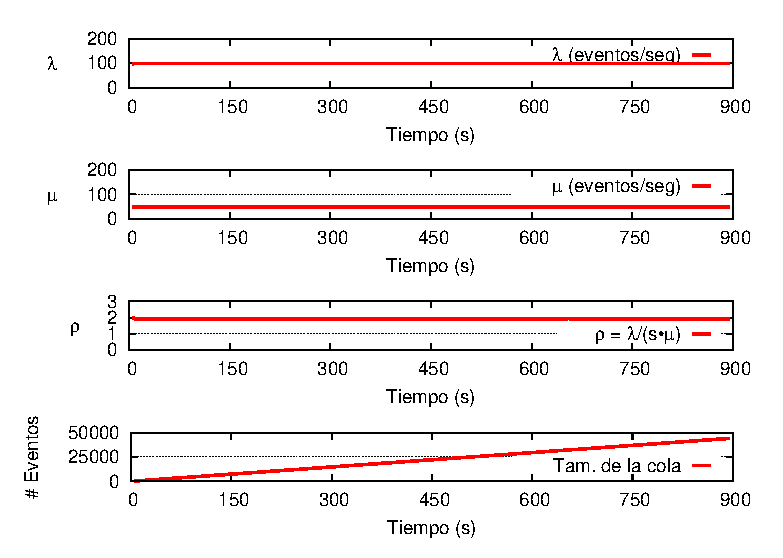
\includegraphics[scale=1]{images/exp/app3/sm/logical/statusOnePE.eps}
    \caption{Estadísticas del primer PE en la tercera aplicación con un envío constante de la fuente de datos sin uso del modelo.}
    \label{fig:app3-statusOnePE-sm}
\end{figure}

\begin{figure}[!htp]
\centering
	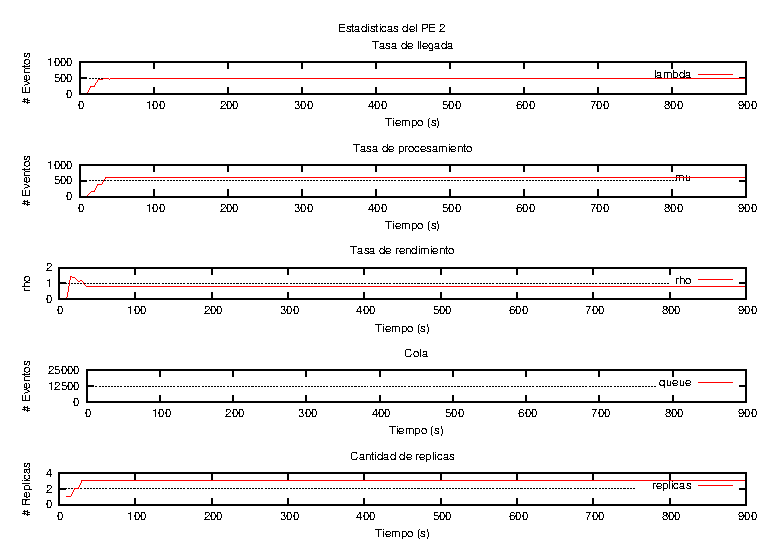
\includegraphics[scale=1]{images/exp/app3/cm/logical/statusTwoPE.eps}
    \caption{Estadísticas del segundo PE en la tercera aplicación con un envío constante de la fuente de datos con uso del modelo.}
    \label{fig:app3-statusTwoPE-cm}
\end{figure}

\begin{figure}[!htp]
\centering
    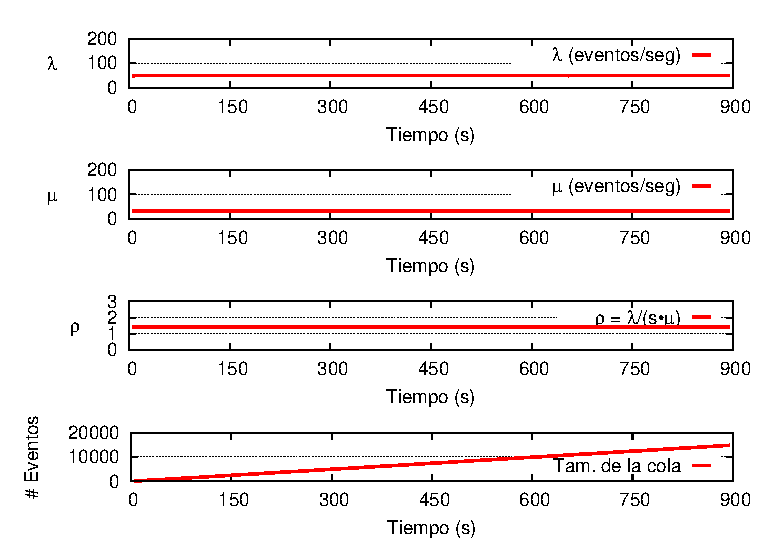
\includegraphics[scale=1]{images/exp/app3/sm/logical/statusTwoPE.eps}
    \caption{Estadísticas del segundo PE en la tercera aplicación con un envío constante de la fuente de datos sin uso del modelo.}
    \label{fig:app3-statusTwoPE-sm}
\end{figure}

\begin{figure}[!htp]
\centering
    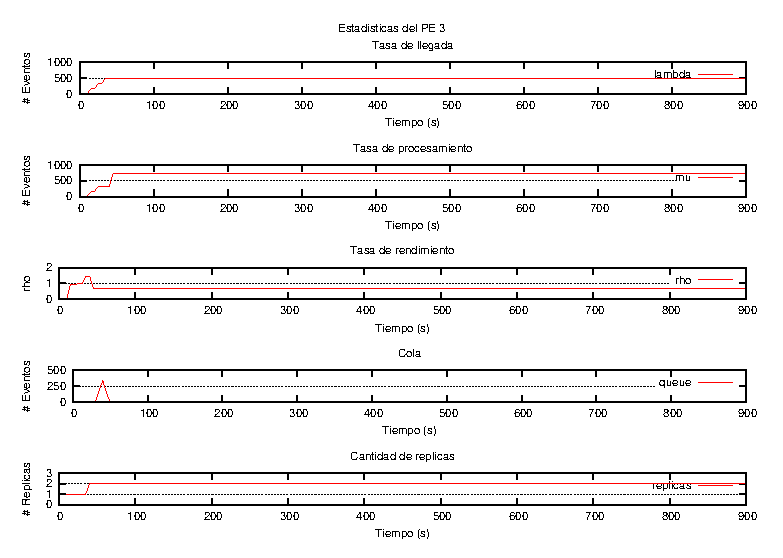
\includegraphics[scale=1]{images/exp/app3/cm/logical/statusThreePE.eps}
    \caption{Estadísticas del tercer PE en la tercera aplicación con un envío constante de la fuente de datos con uso del modelo.}
    \label{fig:app3-statusThreePE-cm}
\end{figure}

\begin{figure}[!htp]
\centering
    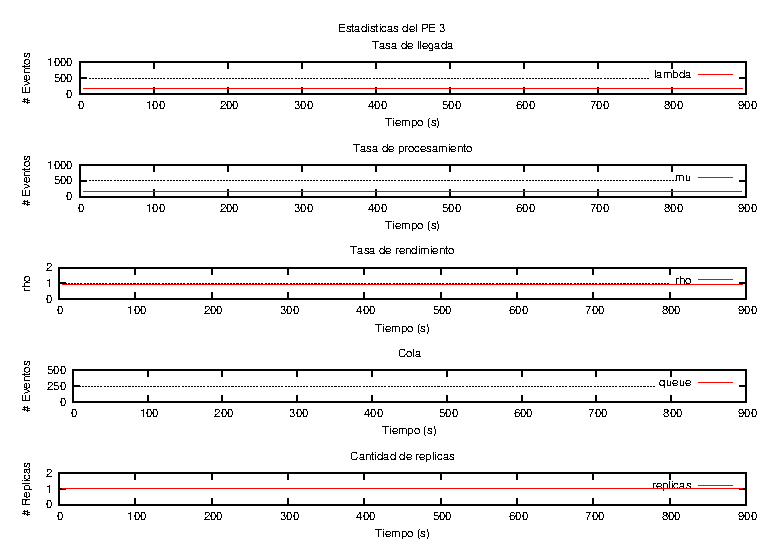
\includegraphics[scale=1]{images/exp/app3/sm/logical/statusThreePE.eps}
    \caption{Estadísticas del tercer PE en la tercera aplicación con un envío constante de la fuente de datos sin uso del modelo.}
    \label{fig:app3-statusThreePE-sm}
\end{figure}